% Requirements Analysis
%
\chapter{Requirements Analysis}

This chapter establishes the objectives and requirements of the present work. To provide a clear specification for the developed solution, the requirements are derived systematically through a step-by-step analysis based on the following.

\section{Research Aim and Questions}

The overall aim of this thesis is two-fold. It is to first understand the influence of power amplifier nonlinearity on the power amplifier chain of the SSR-X (INTRODUCE ABBREVIATION, ASK PROF HENSEL) pulse compression radar, and secondly, to counteract these effects using digital predistortion. These nonlinearities generally compound as input power increases towards saturation. Digital predistortion can counteract these effects, enabling the power amplifier to run closer to saturation without violating regulations and a significant performance degradation. This keeps the radar spectrally compliant and enables the radar to accommodate higher power and consequently higher SNR. This increased SNR headroom enhances detection probability of the radar. For instance, this headroom can be used to increase radar detection range or detect targets with a smaller cross section at the same range – such is a direct performance gain. SNR at the output of the system is increased without the need for purchasing additional expensive hardware. Mitigating nonlinearity effects may also aid in shrinking range sidelobes around strong targets, recovering the ability to detect weaker targets close in their vicinity. Moreover, if the sidelobe level reaches a certain threshold, false targets may emerge – misleading navigators. Mitigating such effects is paramount to improving radar performance and reliability. Specific research questions pertinent to the overall objective are outlined below:

\begin{itemize}
    \item \textbf{RQ1:} What are the effects of power amplifier chain non-linearity on the SSR-X pulse compression radar performance?
    \item \textbf{RQ2:} What existing models best emulate the power amplifier chain non-linearity effects on the SSR-X pulse compression radar?
    \item \textbf{RQ3:} What digital predistortion techniques exist to counteract the non-linear effects of the power amplifier chain?
    \item \textbf{RQ4:} To what extent can digital predistortion counteract the non-linear effects of the power amplifier chain and improve performance?
\end{itemize}

\section{System Environment}

\begin{figure}[tb]
  \centering
  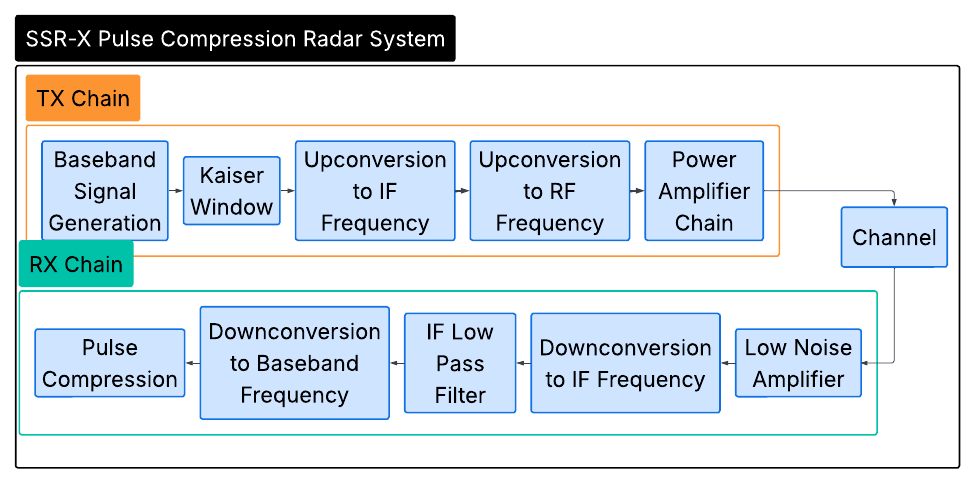
\includegraphics[width=0.9\textwidth]{images/SSR-X Pulse Compression Radar System}
  \caption{SSR-X Pulse Compression Radar System}
  \label{fig:pulse_compression_radar_system}
\end{figure}

This section describes the hardware environment of the SSR-X pulse compression radar system. The system is confined to the pulse compression radar chain of the SSR-X radar transceiver (ABBREVIATION, ASK PROF HENSEL), shown in Figure~\ref{fig:pulse_compression_radar_system}. A radar pulse signal is generated in the transmit chain and then input into the power amplifier for signal amplification before transmission. The echo of this pulse is then captured by the receive chain after some delay and attenuation. Pulse compression is performed at the end of the signal chain to increase SNR, increase range resolution, and determine range of a detected target. The thesis work focuses on investigating the nonlinear effects the power amplifier chain has on the system and finding a suitable digital predistortion solution to correct for these effects. 

\section{Stakeholders}

The stakeholders of this thesis are those who influence the direction of work and benefit from its results. They are outlined below along with their interests:

\begin{itemize}
    \item \textbf{NACOS Marine Radar Developers:} The engineers at NACOS Marine, who are responsible for the maintenance and development of the radar system, benefit from the results of this work, as it will provide insight on what the effects of power amplifier nonlinearity have on the radar system and its performance. It will help them understand the extent of these effects and how they may be detrimental to the overall radar system performance. The work may also provide potential solutions to these issues – guiding engineers in improving the quality and performance of the product they are developing.
    \item \textbf{NACOS Marine Product Management:} The product management department at NACOS Marine may benefit from this work, as it may improve the performance of the product they are selling. Higher performance – increased target range or detection of smaller targets – may open new market potential, increasing sales and revenue of the product. 
    \item \textbf{International Electrotechnical Commission (IEC) Technical Committee:} According to the International Standard IEC 62388, X-band maritime radar shall transmit within the confines of the allocated band 9.2-9.5 GHz \cite[Sec.~6.2.1.1]{iec62388}. IEC are interested in the compliance of this requirement. Power amplifier nonlinear effects may result in unwanted emissions spreading outside of the confined frequency band – violating this requirement. This thesis work may present solutions to countermand these effects, ensuring spectral compliance with the standard.
    \item \textbf{Radar System Users:} Users of the radar system, namely crew members responsible for navigating their vessel at sea, are interested in the results of this thesis, because it will potentially improve performance and reliability of the radar image used for navigating safely. The solutions presented in this thesis may aid in reducing masking around strong targets – enabling weaker targets within their vicinity to be distinctly detected. There is also the risk of the emergence of false targets – which this work may potentially mitigate. This helps crews to be sure that they can trust their navigation instruments. Performance gains, such as increased range and detection of smaller targets, may also help crews navigate more safely to avoid collision.
    \item \textbf{The Student:} The student, the author of this thesis, is interested in learning about the technicalities of radar development and deepening their understanding of concepts in signal processing. This thesis work provides the student the opportunity to gain practical experience in these aspects.
\end{itemize}

\section{Objectives Analysis}

The overarching objective of this work is to determine what real effects power amplifier nonlinearity has on the pulse compression radar system and appropriate predistortion techniques to amend such effects for performance gain and spectral compliance. To better solidify how this can be achieved, it is divided into several detailed objectives below.

\subsection{Generic Modelling of the SSR-X Pulse Compression Radar}

The first objective is to develop a pulse compression radar simulation that can be used as a controlled platform for nonlinearity and digital predistortion experiments. This simulation serves as a generic model to understand the general behaviour of the power amplifier chain and apply different parameter values and view how this affects the outputs. Within such a simulation, various power amplifier nonlinearity models from literature can be dynamically applied and their effects investigated. On that note, a simulation will also demonstrate what the outputs of an ideal system would be, void of nonlinear effects. Furthermore, the simulation forms the basis for experimenting with different digital predistortion algorithms. 

To best understand the power amplifier chain behaviour, it stands to reason for the simulation to simulate the main stages of the pulse compression radar and pulses generated by the real system in its standard operating mode. The pulses used by the pulse compression radar comprise a medium and long pulse – chosen depending on desired range. These pulses are generated in the real system’s FPGA as baseband signals. They are then windowed, upconverted to IF frequency, converted to analogue signals, then upconverted to RF frequency preceding amplification for transmission. This forms the transmit chain. Each pulse would return an attenuated and time delayed echo then passed through the receive chain of the system. In the receive chain, the echoes are amplified, down converted back to IF and baseband frequencies, and low pass filtered at the IF frequency. The final stage of the chain entails pulse compression to maximise SNR and detect after which delay time the echo returns. Each of the above stages act as primary components forming the pulse compression radar system.

Furthermore, the simulation should produce plots that can be used to quantitively analyse power amplifier nonlinearity effects. Plots relevant to this topic are namely spectra of the various signals across the chain, AM-AM and AM-PM curves of the power amplifier, and the pulse compression output. Therefore, it stands to reason for the model to generate said plots. To evaluate overall performance, relevant plots should include quantitative values for KPIs pertinent to known nonlinearity effects – these primarily encompass signal magnitude, side lobe level, harmonics level, AM-AM linearisation, and AM-PM phase deviation. To elaborate, pulse compression and spectrum plots should measure main lobe peak amplitude, peak side lobe level (PSL), and integrated side lobe level as metrics to determine effects on signal magnitude, spectral compliance and range side lobes. Spectrum plots should additionally measure main lobe level of the second harmonic to determine extent of harmonics’ effects. AM-AM curves should measurably highlight the linear range extension as a KPI for linearisation effect, whereas total phase deviation should constitute the KPI for AM-PM curves. 

This objective is achieved if the simulation is developed and supports both pulses and the experimentation of power amplifier nonlinearity and digital predistortion models – involving the generation of relevant simulation plots with quantitative values for KPIs. 

\subsection{Precise Modelling of the SSR-X Pulse Compression Radar}

Following completion of the generic pulse compression radar model, the second objective is to adjust the parameters of the simulation to best model the actual pulse compression radar hardware. This will allow experiments on the nonlinearities and digital predistortion to be relevant to the real-world system. This will result in understanding the actual effects nonlinearity has on the pulse compression radar system hardware and how it reduces performance.

This objective involves performing lab measurements on the pulse compression radar hardware to obtain an understanding of real system behaviour. The measurement step should endeavour to produce any relevant plots that help determine accurate parameters and settings for the simulation. The plots that can be realistically derived from measurement are dependent on the confines and available connectors of the hardware. Hence, it is unrealistic to obtain all the same plots generated by the simulation. 

When sufficient measurement plots and values are obtained, simulation parameters can be finetuned to emulate the hardware as closely as possible. The simulation should thus ideally include a variety of power amplifier nonlinearity models, so a comparison can be made between models to determine which best matches the real system. This is conducive to understanding the actual nonlinearity effects on the hardware and deducing its effects on performance.

This objective is achieved when adequate measurements for behavioural understanding are obtained and the simulation finetuned with the best matching power amplifier model chosen to precisely emulate the power amplifier chain hardware. 

\subsection{Implementation of Digital Predistortion}

Once concrete nonlinear effects are determined from the precise model, the final objective involves implementing digital predistortion to counteract these effects and improve performance. This would involve the application of digital predistortion algorithms in the simulation, where the counter-effects on nonlinearity can be observed in the generated simulation results. To compare and evaluate results, it stands to reason to generate three separate sets of results – one ideal, one with nonlinear effects modelled, and one with digital predistortion applied. Values of the curves’ KPIs – signal magnitude, side lobe level, harmonics level, AM-AM nonlinear deviation, and AM-PM phase deviation – can then be directly compared. This aids in providing a metric to quantitively evaluate the extent of performance gain digital predistortion introduces.  This same comparison and evaluation could potentially also be performed on the real pulse compression radar hardware by implementing the simulated digital predistortion algorithm in its firmware.

This objective is achieved when a digital predistortion algorithm is implemented in the simulation (and possibly in the firmware) and ideal, nonlinear, and predistorted results are compared with subsequent performance gain evaluated.  

\section{Requirements Overview}

Based on the system environment and analysis of stakeholders and objectives, the following functional and non-functional requirements are derived. Functional requirements describe behaviours that the system must provide, whereas non-functional requirements describe that quality constraints the system must adhere to e.~g. performance, reliability and usability. These requirements must be concrete and testable to determine whether the developed system has truly fulfilled them. The requirements directly impact decisions on system design and final evaluation.

\subsection{Functional Requirements}

\textbf{FR1:} The pulse compression radar simulation shall include the following modular stages for complete modelling of the real system: 
\begin{itemize}
    \item Baseband signal generation
    \item Baseband signal windowing
    \item Up conversion to IF frequency
    \item Up conversion to RF frequency
    \item Transmit chain amplification (power amplifier)
    \item Channel effects (delay and attenuation)
    \item Receive chain amplification
    \item Down conversion to IF frequency
    \item IF frequency low pass filter 
    \item Down conversion to Baseband frequency
    \item Pulse compression
\end{itemize}
 
\textbf{FR2:} The pulse compression radar simulation shall include the medium and long pulses generated by the real system respectively.

\textbf{FR3:} The pulse compression radar simulation shall apply at least two known power amplifier nonlinearity models for comparison.

\textbf{FR4:} The pulse compression radar simulation shall apply at least one known digital predistortion algorithm for evaluation.

\textbf{FR5:} For each transmit pulse type (medium and long), the pulse compression radar simulation shall generate analysis plots that overlay the ideal, nonlinear power amplifier, and predistorted power amplifier cases for direct comparison.

\textbf{FR6:} Generated pulse compression radar simulation spectrum plots shall include quantitative values for the following KPIs for evaluation:
\begin{itemize}
    \item Main lobe peak amplitude
    \item Peak side lobe level (PSL)
    \item Integrated side lobe level (ISL)
    \item Second harmonic main lobe level
\end{itemize}

\textbf{FR7:} Generated pulse compression radar simulation pulse compression plots shall include quantitative values for the following KPIs for evaluation:
\begin{itemize}
    \item Main lobe peak amplitude
    \item Peak side lobe level (PSL)
    \item Integrated side lobe level (ISL)
\end{itemize}

\textbf{FR8:} Generated pulse compression radar simulation AM-AM plots shall include quantitative values for the KPI of linear range extension for evaluation.

\textbf{FR9:} Generated pulse compression radar simulation AM-PM plots shall include quantitative values for the KPI of total phase deviation for evaluation.

\textbf{FR10:} Measurements on the pulse compression radar hardware shall be performed to understand real system behaviour and precisely finetune the simulation.

\subsection{Non-Functional Requirements}

\textbf{NFR1:} The pulse compression radar simulation shall be developed in Python to ease the learning curve and development speed for the student.

\textbf{NFR2:} The pulse compression radar simulation shall be developed modularly, so that it can be easily maintained and extended.

\textbf{NFR3:} The documentation and implementation of the work shall be well structured and comprehensible to ensure future developers or researchers can inspect, reproduce, or extend the work. This entails clear project structure, fully documented project components, and repletely annotated results.  